

\chapter{介绍} \label{chap:chap1}
\section{概要}
这本书探讨了针对灵长类动物前额叶皮层基本功能的定义,本章将解释为什么我们采用比较定义的方法来解决这个问题。同时,我们还将补充说明为什么定义基本功能的方式要依赖于对大脑皮层区域之间连接差异的理解。由于我们的研究基于细胞记录、影像激活和大脑病变等三种情况,本章将解释这些方法如何相互关联,并综合考虑它们的优缺点。我们强调了成功的灵长类前额叶皮层理论必须遵循以下几个先决条件:该理论必须涵盖广泛的发现,必须说明前额叶皮层的功能与其他皮层区域不同,必须解释前额叶皮层的优势,必须明确说明前额叶皮层作为一个整体的功能以及其功能必须能够被测试。

\section{介绍}
在这本书中,我们首先提出灵长类动物的前额叶PFC可以实现的基本功能:可以利用当前行为环境的信息,根据当前的生物的需求产生目标活动。PFC是如何执行这一功能以及它如何精准的执行功能是这本书的两个关键主题。当然,我们很清楚,很多书和文章都涉及这些主题,但这本书的不同之处在于还有另外两个问题:为什么前额叶皮层会理解做它所做的事情,以及它是如何做到的它要实现的事。
\par 
生物学针对问题需要做出两个方面的回答,例如在危险情况下为什么心率会加速。一方面,是基于生理机制,大脑检测到危险并产生自主输出。另一方面,基于生物进化史,我们的大脑、心脏和循环系统在保持其本来面貌的同时也会进行维持和调整,这样生理和发育系统都会导致心率加速。

\par 
Tinbergen阐述了这个概念\cite{tinbergen2020study},提出我们对任何生物系统应该思考的四个问题:
它是如何进化的(系统发育)?
它是如何促进适应(选择)?
它是如何成长(个体发育)?
以及它是如何工作的(机制)?
关于前额叶皮层的文章通常会处理最后两个问题,但很少会解决前两个问题。
然而,我们认为这两个问题是理解前额叶皮层的关键。
\par 
当然,神经科学家可以说,他们对进化或适应不感兴趣。
但我们认为他们这样做犯了一个策略错误。
正如第二章所解释的那样,PFC 的一些部分首先出现在早期灵长类动物中,其他部分则出现在灵长类动物的进化中。
忽视这段历史,神经科学家会对前额叶皮层的研究失了一些重要的见解。
\par 
事实上,我们是类人猿的灵长类动物,是类人猿、人类和猴子的最后一个共同祖先的后代。
我们看到的世界就像任何其他的类人猿一样,事通过一个中央凹看到的世界在精致的细节,像大多数类人猿一样是全彩的。
其他种类的哺乳动物,甚至其他种类的灵长类动物,都缺乏这些视觉专门化。
与其他哺乳动物相比,我们的嗅觉和味觉和听觉能力都不佳。
但我们对这个世界的了解与其他哺乳动物不同——而且更有效。
PFC不仅是理解我们如何做到这样做的关键,而且也是理解这是如何发生的关键。

\section{目的}
针对本文研究的两大主题,我们针对性的提出了五个目标,并在这本书中明确地说明了我们想要实现的目标。分别是:
\par 
  1.说明灵长类动物PFC是如何进化的,以及PFC给灵长类动物带来了什么优势。 
\par 2.说明灵长类动物的神经连接是如何定向到PFC,而不是其他大脑皮层区域来执行所需要实现的功能。 
\par 3.对灵长类动物PFC的基本功能提出一个具体的定义。
\par 4.在基本功能的定义下,解释当人们在执行复杂的认知任务时,大脑皮层产生的成像结果。
\par  5.告诉读者我们的定义与其他文献中的不同,以及我们该如何对其功能进行测试。
\par 
这些目标都很重要。我们考虑当忽略第一个问题会产生什么结果?
为了实现这一点设想,我们需要了解不同哺乳动物物种的皮质区域之间的同源性。
关于PFC功能定义的两种流行观点认为:PFC的基本功能是工作记忆\cite{goldman1996prefrontal}或监测工作记忆中的项目\cite{petrides1996specialized}。
这些功能被归因于PFC的一部分,正如第\ref{chap:chap2}章所解释的,这是专门在灵长类动物中进化的,而非灵长类哺乳动物的。
\par 
有人可能会认为,没有PFC这部分同源物的动物将会缺乏工作记忆或监测其内容物的能力。
然而研究结果显示并非如此,例如老鼠可以学习径向分支迷宫任务。
实验者用食物颗粒代替迷宫的八个分支,饥饿的老鼠只需全部访问一次分支,就可以来学习到收集颗粒的路径\cite{olton1982disconnection}。
老鼠可以学习分支迷宫任务的事实表明,它们可以记住和监测它们的哪条分支之前访问过。
因此,一个全面的理论必须解释:为什么灵长类动物需要它们的PFC的某些部分来完成,其他哺乳动物在没有这些区域的同源物的情况下也可以学习和执行的任务。
\par
我们的第二个和第三个目标特别重要,因为与大脑的其他部分相比它们处理PFC的特定功能,。
如果灵长类动物的部分PFC进化出来了,我们需要了解这些区域可以做什么,而大脑的其他部分不能做什么。
如果缺少这部分的分析,就破坏了其他几种理论。
例如,工作记忆\cite{baddeley1998domain}、全局工作空间理论\cite{dehaene1998neuronal}和多重需求理论未能区分PFC和后顶叶皮层的作用,在该理论中这两个皮质区域都有助于这些功能。
所以这三种理论都归因于PFC的功能,是因为其他区域也有作用。
然而,理解灵长类动物PFC的关键:在于理解其功能与皮层的其他部分的不同。
\par
我们的第四个目标需要理解我们提出的PFC的基本功能是如何解释当人们执行复杂的认知任务时大脑产生的成像结果。
大脑执行的任务如此之多,一个简单的叙述似乎没有希望。
人们可能会问,一个简单的功能,无论多么基本,是如何解释复杂认知过程中的成像结果呢?
\par
我们的第五个也是最后一个目标似乎与其他目标不同,但它也同样重要。
其他文献中的许多定义都很笼统,以致于它们永远无法被驳倒。
举个例子,PFC的执行功能几乎没有提供什么可验证的假设,也没有论证是否有任何不涉及执行功能的重要行为。
与一些关于PFC的理论不同,我们提出的观点应该很容易被反驳:人们只需要证明大脑的其他部分执行了我们提出的功能,或者灵长类动物的PFC没有执行这种功能。
\par
我们的五个目标决定了这本书的结构。
第 \ref{chap:chap2} 章讨论了第一个目标:探索灵长类动物PFC的进化。
第 \ref{chap:chap3}-\ref{chap:chap7} 章提出了第二个目标,那就是说明灵长类动物的神经连接是如何定向到PFC,而不是其他大脑皮层区域来执行所需要实现的功能。
第三个目标是关于PFC作为一个整体的功能,因此第 \ref{chap:chap8}章提出了这本书的提案。
第 \ref{chap:chap9} 章通过检查人类脑成像文献来探讨第四个目标。
第 \ref{chap:chap10}章实现了我们的第五个也是最后一个目标,通过比较我们的定义和其他突出的想法和定义进行比较,以及提出如何对我们的定义进行测试。
\par
我们希望任何了解基本神经解剖学的神经科学家都能理解这本书,但我们不认为他们对PFC或用于研究研究PFC的方法有任何专业知识背景。
因此,本章的其余部分提供了一些关于术语的背景材料和一些关键的方法要点。



\section{定义和术语}
\subsection{PFC定义}
甚至连专家有时也会轻率地使用额叶这个词。
当提出“额叶功能之谜”时,指的是前额叶皮层,而不是整个额叶皮层\cite{teube1964riddle}。
在1936年一次演讲之后的讨论中,神经学家斯坦利·科布提出了以下抗议\cite{fulton1932relation}:
\par
我可以说一下这个命名法吗?
这完全混淆了一些概念,这种误解主要是由于缺乏对术语的精确使用。
当我在这里听作者和讨论者的交流时候,我听他们说额叶被切除了,意味着前三分之二被切除了。
我听说运动区过去是三种不同的东西,运动前区域和锥体束同样松散地使用。
这种口语化的表述可能很亲切,但不科学!
\par
我们把这些术语的划分带到心脏,所以我们区分了额叶皮质和额叶的运动区。
我们只在指整个额叶或指额叶皮层的病变时使用额叶一词,这些病变可能侵犯或削弱了运动前区域。
\par
我们也大大区分了前额叶皮层的颗粒状部分和非颗粒状部分。
大脑皮层的类型可以根据内部颗粒层,第 4 层的细胞体的数量和密度进行分类。
颗粒状区域有一个明显的层;颗粒状区域有较少的细胞体浓缩成第 4 层。
当然,这是过于简单化了,但也很有用。
灵长类动物PFC的最大部分具有颗粒状的细胞结构,因此很多人称之为颗粒状的前额叶皮层。
\par
虽然这本书关注的是颗粒状PFC,但我们包括了PFC内的某些颗粒区域,正如我们的定义。
在关于眼眶和内侧PF皮质的章节中,我们讨论了它们的颗粒状和非颗粒状部分。
在这样做的时候,我们认为这两个区域的颗粒部分赋予灵长类动物的优势。

\begin{table}[htbp] 
	\newcommand{\tabincell}[2]{\begin{tabular}{@{}#1@{}}#2\end{tabular}} %换行指令
	\centering
	\caption{人类和猕猴大脑中的前额叶区域( 括号里是区域号)\label{tab:1_1}}
	\renewcommand\arraystretch{1.5}	%设置表格内行间距
	\begin{tabular}{llll}
		\toprule 
		种类 &区域   &  人类  & 猕猴 \\
		\midrule
		\tabincell{c}{颗粒状 \\ 前额叶皮层}&尾部额叶&尾侧 (8)&精密 (8)\\
		&背内侧额叶 & 额上和内侧皮层 (9)  &额上和内侧皮层 (9)\\
		&侧区9&  额上侧 (9) &额上侧 (9) \\ 
		& 中外侧额叶&  额中回(46) & 主沟(46)\\
		&后外侧额叶 &  尾额中回(9/46) & 尾主沟(9/46)\\
		&腹侧额叶& 额下回(45,47)  & 下凸性(45,12)\\
		&颗粒轨道额叶 &眶面(11),延髓 (13),延髓 (14) &眶面(11),延髓 (13),延髓 (14) \\
		%
		%
		&极前额叶  &额杆 (10)   &额杆 (10) \\
		\midrule
		\tabincell{c}{非颗粒状 \\ 前额叶皮层}&内侧非颗粒状前额叶  & \tabincell{c}{前扣带回 (24)、边缘下 (25) \\边缘前 (32)} & \tabincell{c}{前扣带回 (24)、边缘下 (25) \\边缘前 (32)}\\
		&外侧非颗粒状前额叶 & 尾区13和14和非颗粒状岛叶皮质 & 尾区13和14和非颗粒状岛叶皮质\\
		\bottomrule
	\end{tabular}%
\end{table}%

\begin{table}[htbp] 
	\newcommand{\tabincell}[2]{\begin{tabular}{@{}#1@{}}#2\end{tabular}} %换行指令
	\centering
	\caption{前额区组术语 ( 括号里是区域号)\label{tab:1_2}}
	\renewcommand\arraystretch{1.5}	%设置表格内行间距
	\begin{tabular}{ll}
		\toprule
		区域 & 组成部分 \\
		\midrule
		尾侧前额叶 & 区域 8,包括额叶视区 (FEF)?、后外侧前额叶(9/46区)?  \\
		背侧前额叶 & 中外侧前额叶(46区),外侧前额叶(9区)?,后外侧前额叶(9/46区)? \\
		内侧前额叶&边缘下区(25区),边缘前区(32区),扣带前部区(24区),内侧区9和极前区(10区)  \\
		眶额前额叶 & 粒状和粒状眶皮层(11,13,14),粒状岛皮层  \\
		腹侧前额叶&12/47区和45区?,44区? \\
		外侧前运动皮层 & 背侧和腹侧前运动区\\
		内侧前运动皮层 & 前辅助运动区(preSMA),辅助运动区(SMA),扣带运动区(CMAs)  \\
		前运动皮层 & 外侧和内侧运动前区  \\
		\bottomrule
	\par?:可能包含在一个组中的区域\\
		\par a:人类极前部皮层的内侧部分。
	\end{tabular}%
\end{table}%


\par
表 \ref{tab:1_1} 列出了我们在PFC中包含的区域,表 \ref{tab:1_2} 给出了额叶区域的分组。
书中使用的缩略语清单和词汇表分别列在表\ref{tab:0_1}和表\ref{tab:0_2}。
在这些页面上放一个书签可能会很有用。


\subsection{PFC标记}
为了讨论灵长类动物的前皮层,我们需要采用一种命名惯例。
如图 \ref{fig:1_1}所示,用一个单一的名称来称呼PF皮质的大部分颗粒:FD区\cite{von1947neocortex}。
那不符合我们的目的。
尽管如此,我们展示了他们的地图,以表明颗粒状PFC具有足够的同质性,以至于von Bonin和Bailey将其大部分视为单个区域。

\begin{figure}[!htb]
	\centering
	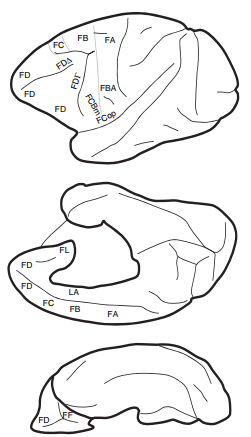
\includegraphics[width=0.5\linewidth]{image_pfc/Fig_1_1}
	\caption{von Bonin和Bailey绘制的猕猴皮层图(1947)。吻侧为左侧,顶部为侧位视图(背侧向上),中间为内侧视图(腹侧向上),底部为腹侧视图(侧侧向上)。请注意,von Bonin和Bailey将大部分前皮层指定为FD区,尽管他们识别了两个颗粒状区域:FF和FL。
		改编自von Bonin G, Bailey P. The Neocortex of Macaca Mulatta,©1947,伊利诺伊大学出版社。\label{fig:1_1}}
\end{figure}
% 必须去除caption后的*,否则交叉引用时会显示?
% 表格和图的\label必须在caption里,否则显示为?

\par
在冯·博宁和贝利的命名法中,一个区域名称的第一个字母代表一个脑叶:F代表额叶,P代表顶叶,T代表颞叶,O代表枕叶,L代表边缘。
最后一个字母表示该瓣内的区域;例如,FA表示额叶区域A,与额叶区域B不同。
\par
布罗德曼简单地按照从大脑顶部到底部的顺序对他的区域进行编号,因为他在一系列水平的大脑区域中遇到了这些区域。
所以4区就是从大脑顶部算起的第四个区域。
有时很容易把冯·博宁和贝利的命名法和Brodmann命名法的两种命名联系起来:例如,区域FA与区域4相当接近。
但有时,冯·博宁和贝利对大脑的看法与布罗德曼截然不同。
\par
如今,通常将这两种命名系统结合在一起,因为它们似乎对某些目的最有用。
“布罗德曼区域”不再需要与布罗德曼自己描述的任何东西相对应,甚至不需要与他想象的任何东西相对应。
\par
除了前额叶皮层的颗粒区和颗粒区外,Brodmann、von Bonin和Bailey等人还发现了介于中间类型的皮层。
颗粒区缺乏的第4层和颗粒区不缺乏的第四层有明显的不同,其他区域具有非颗粒细胞结构。
这种类型的皮质有一个薄的,有时不连续的内部颗粒层。冯·博宁和贝利的区域额叶皮层划分有这个属性。
一些区域,如FCBm(图\ref{fig:1_1}),有更多的中间属性,由字母组合指定。
正如我们前面所说的,颗粒状和非颗粒状前额叶皮层之间的区别代表了一种有用的简化,而不是一种严格的二分法。
使用定量分析法证实:当人们沿着前额皮质的内侧或眶面朝上移动时,第4层变得更厚、更明显\cite{mackey2010quantitative}。
\par
在这本书中,我们使用了一个折中的名字组合。
例如,我们使用字母TE和TEO来表示下颞叶皮层,这是由冯·博宁和贝利引入的。
我们用6号区域作为运动前皮层,就像布罗德曼用的一样。我们使用了各种变体的大杂烩,例如,在Walker\cite{walker1940cytoarchitectural}之后,极性PFC使用了10区。



\subsection{PFC细分}
关于前部皮层的细分还没有达成共识。
正如刚才提到的,冯·博宁和贝利只区分出相对较少的额叶区域,但其他解剖学家已经发现了更多。
例如,通过生成猕猴大脑的结构图(图\ref{fig:1_2}),识别更多的前额叶皮层细分来修改沃克定义的结构图。


\begin{figure}[!htb]
	\centering
	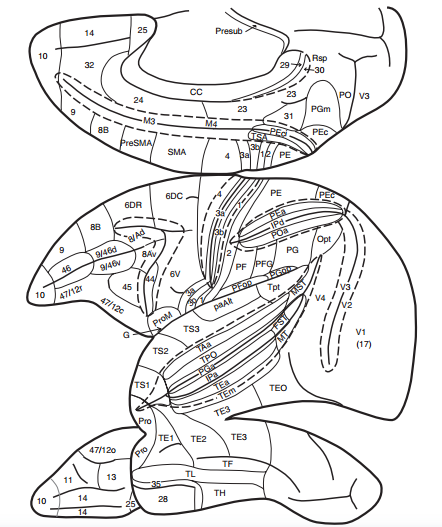
\includegraphics[width=0.5\linewidth]{image_pfc/Fig_1_2}
	\caption{由Petrides和Pandya绘制的猕猴皮层图(2007)。吻侧向左,内侧视图在顶部(腹侧向上),外侧视图在中间(背侧向上),底部腹侧视图(外侧向上)。缩写:CC,胼胝体;G,味觉皮层;Rsp,脾后皮质;Pro,前皮质,新皮质的变体;PreSMA,预辅助运动区;SMA,辅助运动区。区域的细分通常被指定为背(d或d)、吻(r或r)、腹(v或v)、眶(o)、眼(op)、内侧(m)、尾(c)或前(a)。猕猴吻侧前额叶皮层的传出关联通路。神经科学学报,27:11573-86,©2007,美国神经科学学会,已获许可。\label{fig:1_2}}
\end{figure}


\par
通过绘制了人类大脑皮层图(图\ref{fig:1_3}),与他们的猴子大脑皮层图非常吻合\cite{petrides1995impairments}。
然而,Carmichael和Price(1994)对大脑的看法不同\cite{carmichael1994architectonic}。
他们研究了猴子前脑皮层的眶面和内侧表面,发现了比Petrides和Pandya更多的细分,Öngür等人(2003)对人类大脑也做了同样的研究\cite{ongur2003architectonic}。

\par
神经解剖学家发表了相互矛盾的大脑前额叶皮层图,因为他们在是否以及在哪里检测到边界的问题上存在分歧。
在大脑皮层的其他几个部分,神经生理学通过了地形图来帮助定义一个区域。在视觉、听觉和体感进行了区域划分,通常会定义一个区域及其边界。
神经生理学对前额叶皮层没有这样的帮助。同样,不同区域的连接也帮助定义了大脑皮层。
\par
剩下的就是通过加入建筑学知识理解大脑皮层的区域划分,即通过选定的结构特征来识别区域的艺术,称之为皮层建筑学。
当这些区域的特征是依赖于染色的细胞体时,这种做法被称为细胞结构学。
当它们依赖于有髓鞘纤维的模式时,就称为髓结构学。
这两种方法合在一起被统称为皮层建筑学。
退一步说,这是一门不精确的科学。
从本质上讲,皮层建筑学是一种非常高维的模式识别技能,需要多年才能掌握。
因此,几十年来,一种客观、可靠、快速的标记边界的方法一直是皮层建筑学的圣杯。


\begin{figure}[!htb]
	\centering
	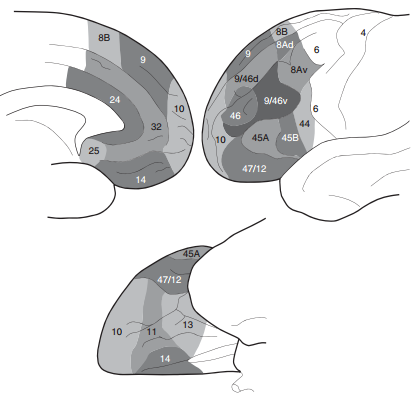
\includegraphics[width=0.5\linewidth]{image_pfc/Fig_1_3}
	\caption{Petrides和Pandya绘制的人类皮层图\cite{petrides1999dorsolateral}。
		在内侧视图(左上),吻侧在右侧;在侧视图(右上),吻侧在左侧;在腹侧视图中(底部),侧面是向上的。
		背外侧前额叶皮层:人类和猕猴大脑的细胞结构分析和皮质连接模式的比较。\label{fig:1_3}}
\end{figure}


\par
Schleicher等人探索了一种他们称之为“观察者独立”的方法\cite{schleicher1999observer}。
他们的意思是,人类观察者不会检测到边界,而是由计算机来检测。
细胞密度从最浅层(第1层)到最深层(第6层)变化。
光密度测量可以反映这种变化,之间的差异反映了不同层中细胞类型和堆积密度的差异。
沿着皮质进行这些测量,加入统计方法可以检测出在不同皮质区域之间划分边界的显著变化。
因此,我们有希望有一天,我们将有一个完整的猕猴皮层地图基于观察者独立的方法,但目前我们还没有找到。

\par
即使可以精确可靠地建立区域边界,它们也可能不对应于功能细分。
例如,在初级运动皮层- Brodmann命名法的4区和von Bonin和Bailey命名法的的FA区-其内侧和外侧的细胞结构不同,内侧的细胞体更大。
但这种特性仅仅是因为内侧运动皮层控制腿部,轴突向脊髓下方延伸,有很大的细胞体。
细胞结构上的差异并不对应于功能上的差异,而是涉及身体不同部位的差异。
如果解剖学家在左脑前部皮层中发现了类似的差异,会将这两个区域标记为单独的区域。
但是,这种区别可能很少或根本没有说明功能。

\par
鉴于在识别前额叶皮层的功能细分方面存在的问题和不一致,我们选择使用一般的描述性术语。
图 \ref{fig:1_4} 显示了猕猴大脑的这些术语;
图 \ref{fig:1_5} 显示了它们与沟和编号区域的关系。

这种方法的优点是不与任何特定的划分图绑定,同时与大多数其他的命名划分图保持一致。

\begin{figure}[!htb]
	\centering
	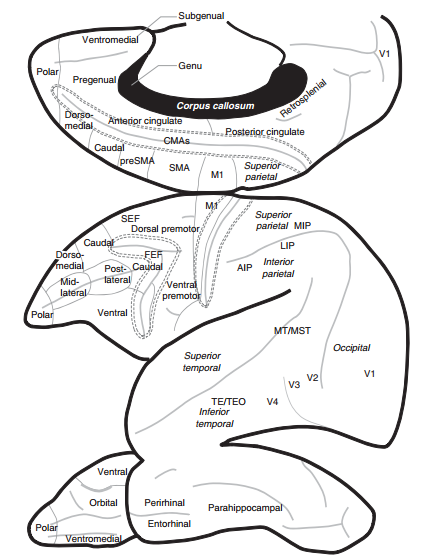
\includegraphics[width=0.5\linewidth]{image_pfc/Fig_1_4}
	\caption{本书中使用的对猕猴大脑的皮层分区的命名分区图。
		格式如图 \ref{fig:1_2} 所示。
		缩略语:参见缩略语列表 \ref{tab:0_1}。\label{fig:1_4}}
\end{figure}




\subsection{约定和缩写}
我们的关于皮层划分的定义主要取决于前额叶皮层的连接解剖学。
因此,当我们回顾成像研究的结果时,我们有时会检查激活的峰值在哪里,以便将它们与我们所知道的猴子的同源区域联系起来。
为了做到这一点,我们使用了\href{http://www.cabiatl.com/mricro/MRIcro/index.html}{MRIcro程序},它采用报告的激活位点坐标,并显示它相对于旋回和沟状地标的位置。
因此,我们对大脑活动定位的描述有时与原作者的不同。
我们希望他们能原谅我们的冒昧。


\subsection{本节小结}
考虑到不同前额叶区域的各种标签,我们请读者参考表 \ref{tab:1_1} 和 \ref{tab:1_2} 进行阅读。
本章中的表格和数字需要注意一下。
在猕猴和人类大脑皮层的某些部分使用相同的名称是很容易的;要确定这些区域就是它们的共同名称所暗含的信息:从共同祖先那里继承的同源物,则完全是另一回事。
第 \ref{chap:chap2} 章主要讨论了这个问题。

\begin{figure}[!htb]
	\centering
	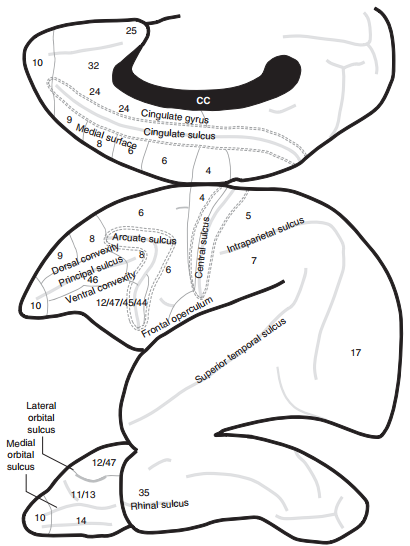
\includegraphics[width=0.5\linewidth]{image_pfc/Fig_1_5}
	\caption{图 \ref{fig:1_4} 中区域命名与皮质区、选定的脑沟和脑回的对应关系图。
		格式如图 \ref{fig:1_2} 所示。
		缩写:cc,胼胝体。\label{fig:1_5}}
\end{figure}



\section{指纹}
现在我们转向一个关键概念,它是我们第二个和第三个目标的核心。
一个成功的关于前额叶皮层的理论不仅要解释它的作用,还要解释为什么只有前额叶皮层能做到特定的目标。
为了实现这些目标,我们依靠“指纹”。
用这个比喻来描述一个极坐标图\cite{zilles2001cyto},该极坐标图显示了皮层区域中各种神经递质受体和转运体的密度。
就像在法医科学中一样,神经递质“指纹”具有基于许多特征的识别功能。
将一个区域的整体连接模式称为其连接指纹\cite{2002Dorsal},正如我们在本章节的研究所做的那样。


\subsection{连接指纹图谱}
关于皮质连接的正式研究始于1969年\cite{pandya1969cortico}以及1970年\cite{jones1970anatomical},并一直持续到今天。
当然,随着方法变得更加敏感和可靠,以及其他原因,结果也会发生变化。
\par
例如,在不同的时间,基底神经节的输出被认为只针对辅助运动区(SMA)\cite{schell1984origin};
同时针对初级运动皮层(第4区)和前运动皮层(第6区)\cite{kemp1971connexions};
或瞄准其他区域,包括前辅助运动区(preSMA)、扣带运动区(CMAs)和颗粒状前部皮层\cite{matelli1996thalamic,mcfarland2002thalamic}。
最近的证据表明,基底神经节的输出也延伸到顶叶\cite{clower2005basal}和颞叶\cite{middleton1996temporal}。
毫无疑问,人们所接受的解剖结构总有一天会再次改变,但现在我们只能将按照现有的结果继续研究。
\par
皮质区域的连接指纹具有重要的作用,连接指纹很大程度上限制了相关区域的功能。
例如:如果没有视觉输入,皮质区域就不能执行视觉功能。
利用解剖学数据库中的数据绘制了前额皮质不同部分之间的连接图\cite{2002Dorsal}。
该数据库名为\href{http://www.cocomac.org/}{Cocomac},是指猕猴的实际连接。
在最新的版本中,它包含了来自413项研究的39,748个连接条目的数据。
\par
利用这些连接数据研究\cite{2002Dorsal},实验结果表明每个前额叶区域都有一组独特的输入和输出。
对于每个前额叶区域,他们用极坐标绘制出连接的强度。
图\ref{fig:1_6}显示了两个相连的指纹,一个位于前部前部皮层的背部(区域9),另一个位于眶前部前部皮层的内侧(区域14)。
周长表示与特色区域相连的区域,半径表示每个连接的主观强度,范围从1到3。

\par
Passingham等人也使用多维尺度来研究这些联系\cite{2002Dorsal}。
如图\ref{fig:1_7} A所示,多维缩放显示没有两个区域具有完全相同的连接模式。
最近也使用Cocomac数据库绘制了各个前额叶区域的远距离皮质-皮质连接图\cite{averbeck2008statistical}。
他们证实,每个前额叶区域都有独特的连接模式。

\par
大脑的任何一个区域都不是单独活动的,所以我们需要把前脑皮层的每个部分作为一个整体来理解。
因此,继续使用分层聚类分析来表明\cite{2002Dorsal},在前额叶皮层内,人们可以识别具有相似连接的区域簇。
使用了一种不同的技术来定义这样的集群,并得出了类似的结论\cite{averbeck2008statistical}。

\par
图\ref{fig:1_7} B显示了PFC内的五个簇\cite{2002Dorsal}。
与Averbeck\cite{averbeck2008statistical}的分析一样,不同簇的功能完全取决于连接。
然而,当人们将这些基于连接的集群与前脑皮层中每个区域的位置信息结合起来时,就会出现一个略有不同的观点。
出于这个原因,我们使用了一个与Price\cite{price2010neurocircuitry}提出的方案非常相似的方案。
他们识别出前额皮质的五个部分:内侧、眶部、尾部、背侧和腹侧。
第\ref{chap:chap3}-\ref{chap:chap7}章逐章考虑这五个区域,图\ref{fig:1_8}说明了它们。
在很大程度上,这些划分与传统的关于前脑皮层的观点一致。

\par
例如,图\ref{fig:1_7} A支持猕猴的极性前部皮层包含在内侧前部皮层中。
每个区域都是一个更大的区域网络的一部分,包括前运动皮层、顶叶皮层、颞叶皮层和海马皮层。

\par
关于广泛的分布式神经网络的发现带来了挑战,这与我们的第二个和第三个目标有关。
在网络中放置前额叶区域是不够的,还需要说明该区域与同一网络中的其他区域在哪些方面不同。
以神经网络为例,它包括中外侧前部皮层(46区)以及后顶叶皮层的几个部分。
这两个神经网络的病变会对行为产生截然不同的影响。

\par
延迟交替任务的经典版本要求猴子学会在一次试验中选择左边的食物井,在下一次试验中选择右边的食物井,以此类推,从而从一次试验到另一次试验交替进行。
中外侧前部皮层(46区)受损的猴子无法重新学习这项任务\cite{butters1969retention},但后顶叶皮层受损则没有影响\cite{ettlinger1966tactile}。
解释必须是,尽管中外侧前部皮层和后顶叶区共享许多连接,尤其是彼此之间,但它们并不是共享所有的连接。
每个区域的连接指纹导致了重要的差异。


\begin{figure}[!htb]
	\centering
	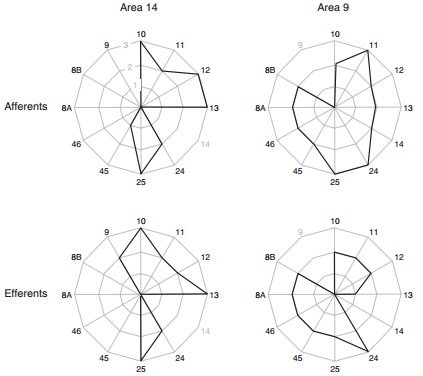
\includegraphics[width=0.5\linewidth]{image_pfc/Fig_1_6}
	\caption{背内侧前部皮层(9区)和部分眶前部皮层(14区)的连接指纹图谱。
		每个极坐标图显示了周边与区域9或14相连的区域,并主观评估了沿半径的投影强度:轻(1)、中等(2)或重(3)。
		例如,左上角的图显示,区域14与区域10有“重”连接。
		区域内的投影不包括在内(圆周上的灰色标签)\cite{2002Dorsal}。 \label{fig:1_6}}
\end{figure}

\begin{figure}[!htb]
	\centering
	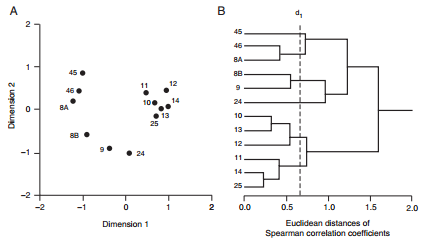
\includegraphics[width=0.5\linewidth]{image_pfc/Fig_1_7}
	\caption{前脑皮层的连接簇图。
		(A)两个连通维度的图,每个点旁边的面积用数字表示。
		(B)沿连接维度的分离分层聚类,记为d1 \cite{2002Dorsal}。\label{fig:1_7}}
\end{figure}


\subsection{生理指纹图谱}
一个区域的连接指纹显示了该区域的约束和功能。通过类推,引入了功能指纹的概念\cite{2002Dorsal}。
他们用生理数据说明了这些特性,所以我们在这里使用生理指纹这个短语。
对于一组数据,他们绘制了细胞活动的五种特性: 
(1)听觉或视觉反应;
(2)本体感觉或皮肤反应;
(3)类似肌肉的活动模式;
(4)活动与运动的时间相关性;
(5)持续的延迟期活动。

\begin{figure}[!htb]
	\centering
	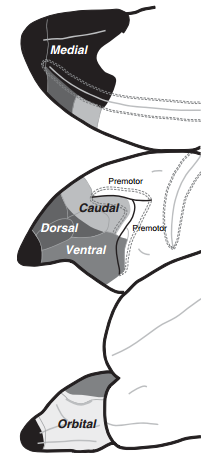
\includegraphics[width=0.5\linewidth]{image_pfc/Fig_1_8}
	\caption{书中用到的前额皮质的五个区域图。
		格式如图\ref{fig:1_2}所示。
		这五个区域中的每一个,内侧(上),眶(下),尾侧,背侧和腹侧前额皮质(中)都是后面一章的主题。\label{fig:1_8}}
\end{figure}

\par
如图\ref{fig:1_9} C显示,SMA和腹侧运动前皮层各细胞类别的相对频率不同。
例如,SMA中较高比例的细胞具有体感觉反应。
图中还显示了两个区域连接指纹的不同(图\ref{fig:1_9} A和B)。
\par
对于第二个数据集,Passingham等人(2002)绘制了细胞对根据记忆或基于视觉线索执行的运动序列的偏好\cite{2002Dorsal,mushiake1991neuronal}。
图\ref{fig:1_10}中的直方图显示了SMA和运动前皮层的结果,活动分为1到7级。
第一类细胞对视觉任务具有完全的特异性;第七类的细胞对记忆引导的任务有完全的特异性。

\begin{figure}[!htb]
	\centering
	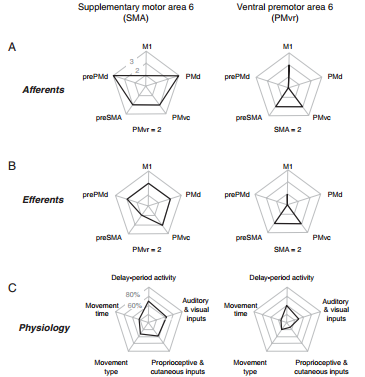
\includegraphics[width=0.8\linewidth]{image_pfc/Fig_1_9}
	\caption{(A,B)辅助运动区(SMA)和腹侧运动前皮层(PMvr)吻侧的连接指纹图谱。
		缩写:M1,初级运动皮层(第4区);PMd,背侧运动前皮层(6区);PMvc,腹侧运动前皮层尾侧(6区);preSMA,预辅助运动区(6区);prePMd,背侧运动前皮层的吻侧部分(6区)。
		每个极坐标图下面的方程给出了SMA和PMvr之间连接的强度。
		(C)同一两个区域的生理指纹图谱\cite{passingham2002anatomical}。	\label{fig:1_9}}
\end{figure}


\par
分类为4表示统计上相等的活动。
SMA显示记忆引导任务的活动优势,而外侧运动前皮层显示相反的偏向。
\par
我们还以生理指纹的形式绘制了这些数据。
图\ref{fig:1_10}顶部的极坐标图显示的数据与下面的条形图显示的数据相同,单元格类沿圆周绘制,每个类中的比例沿半径绘制。

\begin{figure}[!htb]
	\centering
	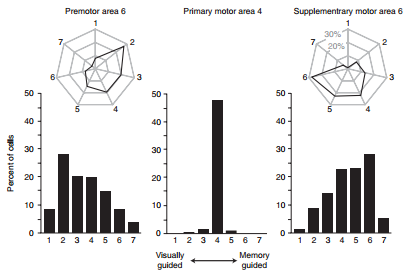
\includegraphics[width=0.8\linewidth]{image_pfc/Fig_1_10}
	\caption{生理指纹显示在运动前皮层(第6区)、初级运动皮层(第4区)和辅助运动区(第6区)对视觉引导和记忆引导的运动序列有选择性对比图。
		第1类细胞对视觉引导序列有完全的特异性。
		第7类细胞对记忆引导序列表现出完全的特异性。
		其他五类细胞表现出中间性质。
		左右柱状图上方的极坐标图显示了与柱状图相同的数据\cite{mushiake1991neuronal}。\label{fig:1_10}}
\end{figure}


\subsection{行为指纹图谱}
到目前为止,我们已经暗示,为了理解前额叶皮层,我们需要比较:通过连接指纹比较区域性质,通过生理指纹比较细胞活动。
从而对行为的理解也会从中加深。
然而,关于前额叶皮层的神经心理学文献往往只强调一些行为任务。
截至2011年,至少有162篇论文发表在对PFC受损的猴子的延迟反应任务上,其中许多论文只涉及这一任务。

\par
这种专注于一个任务有其优势。
例如,它允许在同一任务上进行行为、生理、成像和药理学实验。
但是,仅仅对一个或几个任务的关注可能会导致对左脑前额叶皮层功能的片面看法。
在第 \ref{chap:chap5} 章和第 \ref{chap:chap6} 章中,我们解释了为什么延迟反应任务和它的近亲延迟交替任务会产生这样的歧义。
从这些研究的结果中得出的结论是:如果功能不是唯一的话,前脑额叶层的功能主要是在工作记忆中。
第 \ref{chap:chap10} 章解释了为什么我们拒绝单一前额叶皮层的理论。
但是,人们不需要知道我们为什么这样做,就能理解仅仅依赖少数任务的问题。
在两个任务的基础上得出前额叶皮层在工作记忆中起作用的结论,就像在参观了两个史密斯奶奶苹果园后得出所有成熟的苹果都是绿的结论一样。
\par
灵长类动物前额额叶皮层的病变会对学习和执行这些任务造成严重而持久的损害,或者有些成熟的苹果是绿色的,我们对此并不怀疑。
灵长类动物的前额叶皮层一定有什么东西使得它对这些任务的执行是必要的。
但需要在任务之间进行比较才能理解它是什么。
因此,除了前面讨论的连接指纹和生理指纹外,我们还需要行为指纹,这涉及到任务之间病变效应的比较。
我们需要了解有前额叶病变的猴子在哪些任务上表现出损伤。

\subsection{本节小结}
一个区域的连接指纹会限制了该区域能做什么。
生理和行为指纹可以让我们深入了解这种功能可能是什么。
许多关于前额叶皮层的理论都是从一个或几个任务的发现中发展出来的。
在第 \ref{chap:chap10} 章中,我们将所谓的通用性测试应用于前额叶皮层的理论,检验它们是否能够解释激发它们的任务之外的数据。
为了确定灵长类动物前额皮质的基本功能,我们需要依靠广泛的研究和发现,如连接、生理和行为指纹的缩影。

\section{病变和激活}
鉴于影像成像技术已经使研究完整的人类大脑成为可能。
有人可能会认为,在试图理解前额叶皮层时,我们不再需要诉诸大脑病变的影响。
毕竟,当应用于人类受试者时,影像成像研究比病变研究有两大优势。
首先,大脑皮层激活部分的峰值位于灰质,而在患者中,大脑皮层病变通常会损害潜在的白质。
其次,峰值可以位于特定区域。相比之下,患者的病变通常包括许多不同的区域。


\par
鉴于这些优点,读者可能会奇怪为什么我们如此强调病变的影响。我们这样做是因为对某个区域的活动或激活的观察并没有告诉我们,在没有该区域的情况下,受试者是否无法完成任务。以一项成像研究为例\cite{price1999delineating}。他们的实验对象看到一系列图片,其中一张被指定为目标。
在每次试验中,他们必须从两张图片中选择哪一张与目标有关。
例如,当给他们一把钳子时,他们必须选择扳手而不是锯子。
钳子和扳手在一起是因为它们能抓东西,把它们放在一起需要语义分类。


\par
激活发生在三个地方:左侧颞中皮层、左侧下颞皮层和左侧腹侧前额叶皮层。同时也扫描了一个左腹侧前额皮质完全损伤的病人\cite{price1999delineating}。
病人仍然可以执行任务,即使在任何剩余的前额叶皮质都没有激活。
因此,我们可以得出结论:左腹侧前部皮层对于执行语义分类任务不是必需的,即使它在任务执行过程中显示出激活。
由此我们还可以推断,在腹侧前部皮层没有任何贡献的情况下,中颞叶皮层和下颞叶皮层足以完成任务,我们只有将成像与研究病变的影响结合起来才能得出这个结论。


\par
不幸的是,这种方法很少用于人类大脑研究,因为很难找到只有一个大脑皮层区域病变的患者。
虽然暂时性病变,如重复性经颅磁刺激(rTMS)引起的暂时性病变。
为寻找具有特定病变的患者提供了一种有用的替代方法,但这种方法也有严重的局限性。
人类皮层的大部分深埋在脑沟中,刺激不能选择性地到达它。
此外,刺激效应的精确解剖边界从未为人所知。


\par
由于这个原因,我们的研究在很大程度上依赖于猴子大脑皮层病变影响。
我们可以选择通过使用选择性手术技术,单独切除皮层,而保留底层白质的完整。
人们可以选择性地移除特定区域,特别是在沟槽提供有用指导的地方。
病变的边界可以稍后以合理的准确性评估。作为一种替代方法,人们可以选择性地暂时使某一区域失活。
\par

由于其更高的解剖精度,我们在很大程度上依赖于猴子的实验结果来理解病变效应。
这并不意味着我们完全忽略了对病变患者研究的结果。
这些观察结果可以在几个方面发挥作用。例如,病变对猴子的行为影响可能很难解释,而对人类患者的研究可以帮助解决这些困难。

\par
以两个匹配任务为例。在延迟匹配样本的任务中,猴子首先看到一个物体(样本),在一段时间后,它们必须从两个与样本匹配的物体中选择一个,我们称之为匹配规则。
在延迟的非匹配样本任务中,他们需要选择另一个对象,称之为不匹配规则。

\par
假设前额叶皮层受损的猴子在这些任务中表现有差异。
可能是他们记不住样本,或者无法识别两个物体是相同的还是不同的,也可能是他们不再知道任务规则。
研究前额叶皮层病变患者的一个好处是,我们可以告诉他们规则,然后检查他们是否知道。
如果他们不能正常完成任务,但能告诉实验人员规则,这就证明他们要么忘记了样本,要么在识别两个物体匹配方面存在问题。

\par
这个例子还指出了依赖任务名的危险。匹配和不匹配的任务也被称为“识别记忆任务”。
如果猴子只能以一种方式完成这些任务:记忆和识别物体。
不幸的是,就像在猴子的大脑研究中使用的许多任务一样,这些任务给自己提供了几种替代策略。
猴子可以根据识别、熟悉或最近的情况选择一个物体,这取决于每个实验的细节,有时实验者不知道猴子是如何完成任务的。
具体的比较条件可以区分这些策略,但它们并不总是被使用。
类似地,我们稍后将讨论涉及所谓自定任务的实验。
事实上,是被试还是实验者产生顺序并不重要,所以如果从字面上理解,这个名字可能会产生误导。

\par
然而,只要仔细的解释病变的影像结果,这种方法仍然为一个区域的功能研究提供了一些最重要的证据。
金本位制被称为双重功能解离。
这意味着一个区域的病变会影响一个实验任务的表现,但不会影响另一个实验任务,而其他区域的损伤对两个任务都有相反的影响。
例如,腹侧前部皮层的损伤会破坏猴子执行一种策略任务的能力\cite{baxter2009ventrolateral},而眼眶前部皮层的病变则没有\cite{baxter2007asymmetry,baxter2007orbital}。
相比之下,眼眶前部皮层病变会破坏贬值任务的表现\cite{izquierdo2004bilateral},而腹侧前部皮层病变则不会\cite{baxter2009ventrolateral}。
第 \ref{chap:chap4} 章和第 \ref{chap:chap7} 章详细解释了这些任务及其含义,但即使没有这些细节,我们也可以看到结果建立了某种双重功能分离。

\par
尽管有这些和其他一些例子如 \cite{gaffan2002interaction}指出,这种双重分离在前脑皮层中并不像通常认为的那样常见。
Wilson等人\cite{wilson2010functional}强调,影响整个PF皮质的操作通常比主要影响部分的操作产生更大的影响。
这些发现支持了前额叶皮层作为一个整体工作的观点,第 \ref{chap:chap8} 章讨论了这个话题。

\subsection{本节小结}
在一个以成像实验为主导的领域,许多神经科学家似乎认为,在考虑大脑皮层区域的功能时,对损伤效应的理解几乎没有什么帮助。
我们用影像学文献中的一个例子来反驳这一观点:成像激活显示了信息处理的某些方面,但它们并不像病变研究那样显示出在某些任务或功能中所起的必要作用。


\section{病变与细胞活动}
在本章的前一节中,对比了病变和影像成像方法;以及使用切片对比了病变和细胞记录方法。
这两种方法反映了不同的结果。
正因为如此,病变的成像结果并不总是与发生在同一区域的细胞活动相匹配。
我们在前面讨论了一个例子。
在猴子中,中外侧前部皮层(46区)和后顶叶皮层的损伤有不同的影响,尽管这两个区域彼此相连,并且在各种任务中具有相似的细胞活动。
我们之前提到,中外侧前部皮质受损的猴子无法学习延迟交替任务,而后顶叶皮质受损的猴子则能正常完成任务。
然而,中外侧前部皮层\cite{KOJIMA1984229}和后顶叶皮层\cite{chafee1998matching}中的细胞在延迟期(猴子必须记住执行任务所需的信息的时间间隔)中显示出持续的活动。
结果,中外侧前部皮层的细胞活动和损伤效应非常匹配(持续活动和损伤效应),而后顶叶皮层的细胞活动和损伤效应却不匹配(持续活动但无损伤效应)。

\par
另一个例子是运动前额叶区域的内侧和外侧组,它们具有广泛的相互联系\cite{luppino1993corticocortical}。
内侧区域的病变严重破坏了自我产生的运动,被定义为没有视觉提示的运动。
外侧运动前区病变没有这种影响\cite{thaler1995functions};
相反,它们会影响视觉暗示的动作。
考虑到内侧和外侧运动前区都有许多细胞活动,无论运动是视觉提示还是自我引导,这怎么可能呢?
图\ref{fig:1_10}显示,这两个区域的许多细胞都属于第4类,这表明在统计上,这两种引导形式的活动是相同的。
其他细胞表现出偏见,但它们仍然对两项任务都有显著的活动。

\par
要回答这个问题,我们需要认识到,病变研究的结果告诉我们:在没有病变区域的情况下,大脑的其他区域能做什么,不能做什么。
病变不仅消耗了受损区域的计算资源,还消除了其对其他区域的输入以及其他影响。
在完整的大脑中,当动物进行自我引导运动时,外侧运动前皮层的细胞活动显示出增加的活动(图\ref{fig:1_10}中的5到7类)\cite{mushiake1991neuronal}。
因此,有人可能会认为,外侧运动前区可以在内侧运动前区缺失的情况下接管自发运动。
但假设这些细胞从内侧运动前区接收输入,这些连接产生了5到7类细胞。
然后,在受损的动物体内,这些细胞将不再具有与正常动物相同的特性。
结果是,在内侧运动前区缺失的情况下,外侧运动前区不能“接管”自主运动。

\par
这种解决思路解释了一个原因,即使某些区域在某些行为中没有发挥必要的作用,它们也会表现出活动。
类似的原理也适用于左脑前额叶皮层。
在一个典型的条件视觉运动任务中,一张图片指示猴子做出一种反应,另一张图片指示猴子做出不同的反应。
细胞在中外侧前额皮质和腹侧前额皮质区域编码这些图像反应映射\cite{asaad1998neural}。
然而,这两个区域的病变的影响是不同的。前部前部皮层腹侧的损伤会对这项任务产生严重的损害\cite{wang2000deficit},而前部前部皮层中外侧的损伤只会产生轻微的影响\cite{petrides2019conditional}。
我们可以用与第一个例子相同的方法来调和这些发现。
腹侧前部皮层的病变切断了颞下皮层向中外侧前部皮层的大部分输入\cite{ungerleider1989projections},因此中外侧前额皮质不能“接管”该功能。

\par
基于病变和细胞记录方法的优缺点,我们需要将细胞活动与脑病变的影像结果进行比较,以便从这两种信息来源中获得最大的好处。
\par
书中不时出现的另一种活动是皮层内微刺激。
这种方法通过与研究单个细胞活动相同的电极引入电流。
因此,它至少在数百个细胞中同步产生活动。
与正常发生的放电进行比较是复杂的,但该方法提供了有用的信息,假设它大致模仿正常活动。

\subsection{本节小结}
大脑皮层的病变的影像结果并不总是像人们所期望的那样与细胞活动相匹配。
在本节中,我们解释了出现这些明显不匹配的一个原因。
病变效应和细胞活动都依赖于一个区域的连接,但方式不同。
细胞活动要么反映通过连接接收信息,要么反映一个区域内的信息处理。
因此,这些结果反映了一种行为的神经相关性,而损伤效应则揭示了一个区域对该行为的必要贡献的行为。

\section{细胞活动和激活}
在后面的章节中,我们将讨论大脑皮层区域激活和细胞活动的发现。
然而,由于两个原因,这种组合需要谨慎:血管伪影和细胞活动与成像激活之间关系的不确定性。

\par
首先,血氧水平依赖(BOLD)信号是一种血管信号,因此它对大动脉的位置很敏感。
BOLD信号也可能受到静脉和静脉流出的位置的污染\cite{turner2002much}。
由于这些原因,BOLD信号的峰值与潜在大脑活动的位置只有非常粗略的空间对应关系\cite{kim2004spatial}。

\par
其次,我们对成像激活和细胞活动之间的关系知之甚少。
对猴子的大脑成像和细胞活动进行直接比较会有所帮助,但要想对前额叶皮层的理解有任何价值,这种比较必须针对稀疏编码的网络进行。
在稀疏编码的网络中,附近的细胞具有不同的性质;
在密集编码的网络中,大多数细胞都做着同样的事情。
由于这种相对同质性,密集编码网络(如感觉或运动区域)的结果可能具有误导性。
我们只有少量关于猴子稀疏编码网络的成像数据,如前皮层或海马体\cite{nakahara2002functional,orban2004comparative}。
所以我们必须运用一般的原则来应付。

\par
成像实验了测量BOLD信号。
BOLD反应可以在没有动作电位的情况下发生\cite{logothetis2002neural},当峰值活动不存在时,BOLD信号可以在不同的实验条件下不同。
例如,Maier等人\cite{maier2008divergence}研究了猴子初级视觉皮层的BOLD激活和单细胞活动。
他们使用了一种称为广义闪光抑制的知觉操纵。
当移动的点突然出现在视觉目标刺激周围时,它们抑制了对目标刺激的感知。
抑制性刺激不影响视觉皮层的单细胞活动,但影响了BOLD信号。
这一发现表明BOLD信号对调节效应很敏感\cite{logothetis2008we},这可能是由抑制性突触输入或低于驱动细胞活动阈值的兴奋性突触输入介导的。

\par
一个研究得特别充分的例子涉及小脑。
虽然突触激活和BOLD信号在小脑皮层密切相关,但其输出神经元浦肯野细胞的活动却不是这样\cite{thomsen2004principal}。
浦肯野细胞的突触输入,而不是浦肯野细胞的活性,驱动BOLD信号\cite{gold2002neuronal}。
浦肯野细胞的两种主要输入:攀爬纤维\cite{offenhauser2005activity}和平行纤维\cite{thomsen2009principal}诱导的局部场电位呈线性增加,而这些电位反映的是突触输入,而不是浦肯野细胞的放电活动。


\par
因此,大多数证据支持这样的结论,即成像研究中测量的信号并不直接反映神经元的活动,而是反映突触的输入。
有时净突触输入(激活)与神经元活动相关,但通常并非如此。
因此,我们在本书中将细胞活动与区域活动区分开来。
我们采用激活来反映突触的影响,而不是单个细胞的放电率\cite{logothetis2002neural}。


\subsection{元分析}
我们前面提到了在解释病变效应时过度依赖一个或几个任务的危险。
同样的谨慎也适用于细胞记录和成像。
在一项经常被引用的研究中\cite{funahashi1989mnemonic},猴子盯着一个中央光点,一个线索出现在八个地方中的一个。
经过一段时间的延迟后,一个“开始”的提示触发了眼球跳动到提示位置。
在延迟期间具有显著活性的细胞中,大多数都编码了线索的位置。
可以理解的是,许多神经科学家认为这一结果与细胞编码记忆位置的观点是一致的。


\par
但是,仅仅根据一项任务得出这样的结论是危险的。细胞活动在某种程度上取决于猴子的训练历史。例如,训练猴子区分猫和狗的图片发现\cite{freedman2006experience},在训练过程中,在不同的方向上呈现的刺激比在不同的方向上呈现的刺激有更强的选择性。
这一发现并不令人惊讶,因为动物(和它们的大脑皮层)从经验中学习。

\par
考虑到这一原则,Funahashi等人\cite{funahashi1989mnemonic}的结果为他们的解释提供的支持比他们想象的要少。
如果只研究简单空间记忆任务中的细胞活动,就会发现似乎许多细胞对记忆的位置进行编码。


\par
但我们只能通过比较其他任务中的细胞活动来验证这种印象。
例如,延迟期的细胞活动可能反映了猴子去的地方以及它们记住的地方。
因此,Lebedev等人\cite{lebedev2004representation}训练猴子既记住一个地点,又去别的地方。
在对某个位置表现出选择性活动的前额叶皮层的细胞中,发现百分之六十一的细胞只编码了参与的位置,而在记忆中的作用被排除在外。
只有百分之十六的细胞单独编码记忆的位置,其余的细胞具有混合属性。
只有任务之间的比较才能表明,从空间记忆的角度对神经元活动的解释在很大程度上是错误的。


\par
在第 \ref{chap:chap8} 章和第 \ref{chap:chap9} 章中,我们通过将许多任务的结果制成表格,认识到这种比较的重要性。
表8.1是对猴子损伤效应的汇总,表8.2是对细胞活性特性的选择。
表9.10对人的成像激活做了类似的处理。
只有考虑到一系列广泛任务的结果,人们才能得出关于左脑前部皮层基本功能的结论。

\par
这种方法类似于影像学文献中常用的方法。
由于结果可以在一个共同的解剖坐标框架中报告,因此可以进行元分析,这涉及到从导致某个区域激活的任务中获得的数据的综合。
元分析是生理指纹的另一个名字。


\subsection{本节小结}
虽然第 \ref{chap:chap3}-\ref{chap:chap7}章没有使用极坐标图来说明连接、生理或行为指纹,但它们通过更传统的方式传达了相同的原理。
对于神经解剖学数据,他们在猴子的大脑地图上展示了一个特定区域的连接。
他们强调,了解前额叶皮层需要比较不同大脑区域之间的连接(连接指纹),以及比较损伤效应(行为指纹)和各种任务的活动和激活(生理指纹)。
虽然我们在前言中承认了我们挑选的数据,但我们希望读者会同意我们已经尝试挑选了很多数据集。

\par
本节对比了细胞记录和成像结果。像所有方法一样,成像方法也有局限性。
但与细胞活动研究相比,它至少有三个主要优势:
\par 1.成像技术允许人们同时观察大脑的大部分区域。
\par 2.BOLD信号的峰值位置可能反映了特定功能类型信号的峰值密度,而细胞记录将检测到一种类型的活动,无论它发生在哪里。
\par 3.BOLD信号似乎很好地反映了同步激活。
例如,将脑电图(EEG)和功能成像相结合\cite{parkes2006combining},发现了同步和激活的密切相关性。
BOLD信号与场电位的关系在低频范围内最为密切\cite{kayser2004comparison}。

\par 然而,细胞记录比成像研究有一些优势。
它直接显示了一个区域的信息处理元素所编码的内容。
即使在成像实验中无法检测到不同和混合的神经元群,它也能显示出独特的特性,这对于前额叶皮层这样的稀疏编码神经网络尤其重要。
最后,细胞记录可以区分活动的增加和减少,而成像不能。(成像可以区分活动的增加和减少,但不能区分活动。)对成像文献的讨论很少注意到,例如,激活的增加可能反映了一个区域输出的抑制,这对于稀疏编码的网络尤其如此。


\section{本章小结}
这本书采用对比的方法,以实现对灵长类动物的前额叶皮层的基本功能的定义。它有五个明确的目标:
1.描述PFC赋予的优势;
2.说内部皮层连接如何导致其独特的功能;
3.考虑它如何作为一个整体工作;
4.解释人类进行认知任务期间的大脑激活;
5.解释我们的定义与文献中的其他建议有何不同,以及如何对我们定义的功能进行测试。


\par

为了实现第一个目标,第二章比较了前额叶皮层在不同物种中的发展历程。
为了完成第二个目标,第 \ref{chap:chap3}-\ref{chap:chap7} 章每一章都以对前额叶皮层主要部分的连接的总结开始。
每一章的结尾都简要而具体地介绍了这一部分的功能。
为了实现第三个目标,第 \ref{chap:chap8} 章以第 \ref{chap:chap3}-\ref{chap:chap7} 章的定义为基础,提出了关于前额叶皮层整体基本功能的定义。
为了实现第四个目标,第 \ref{chap:chap9} 章解释了我们如何解释人们执行复杂认知任务时的成像激活。
最后,对于第五个目标,第 \ref{chap:chap10} 章将我们的定义与文献中的其他定义进行比较,提出了一些测试方法,并提出了一些可能与之矛盾的观察结果。



